\documentclass[10pt]{article}
\usepackage[polish]{babel}
\usepackage[utf8]{inputenc}
\usepackage[T1]{fontenc}
\usepackage{amsmath}
\usepackage{amsfonts}
\usepackage{amssymb}
\usepackage[version=4]{mhchem}
\usepackage{stmaryrd}
\usepackage{graphicx}
\usepackage[export]{adjustbox}
\graphicspath{ {./images/} }

\title{KLASY PIERWSZE I DRUGIE }

\author{}
\date{}


\begin{document}
\maketitle
\begin{enumerate}
  \item Udowodnij, że dla dowolnych liczb rzeczywistych \(x, y, z\) zachodzi nierówność:
\end{enumerate}

\[
x^{2}+y^{2}+z^{2}+\frac{3}{4} \geq x+y+z
\]

\begin{enumerate}
  \setcounter{enumi}{1}
  \item Udowodnij, że dla dowolnych dodatnich liczb rzeczywistych \(x, y, z\) zachodzi nierówność:
\end{enumerate}

\[
x^{3}+y^{3} \geq x^{2} y+x y^{2}
\]

\begin{enumerate}
  \setcounter{enumi}{2}
  \item Czworokąt \(A B C D\) jest kwadratem. Wyznacz długość odcinka \(E C\), jeśli \(|A F|=4 \mathrm{i}|F B|=3 \mathrm{i}\) kąt \(A F E\) jest kątem prostym.\\
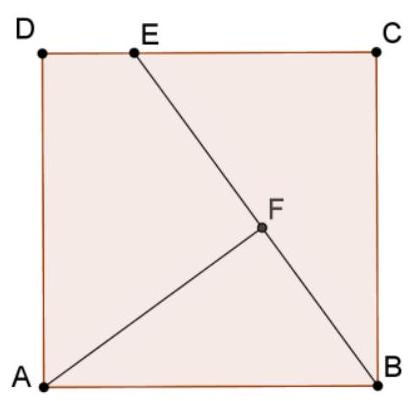
\includegraphics[max width=\textwidth, center]{2024_11_21_59b0c2c0bc9b0a979429g-1}
\end{enumerate}

\section*{KLASY TRZECIE I CZWARTE}
\begin{enumerate}
  \item W okrąg wpisano trapez równoramienny o dłuższej podstawie będącej średnicą okręgu oraz trójkąt, którego boki są równoległe do boków trapezu. Wykaż, że trapez i trójkąt mają równe pola.
  \item Niech \(d_{1}, d_{2}, d_{3}, d_{4}\) będą odległościami punktu wewnętrznego czworokąta wypukłego od jego wierzchołków. Wykaż, że
\end{enumerate}

\[
d_{1}+d_{2}+d_{3}+d_{4} \geq 2 \sqrt{2 S}
\]

gdzie \(S\) oznacza pole czworokąta.\\
3. W trójkącie prostokątnym dane są długości jego przyprostokątnych. Na bokach zbudowano kwadraty, a następnie wyznaczono sześciokąt jak na rysunku. Oblicz pole tego sześciokąta.\\
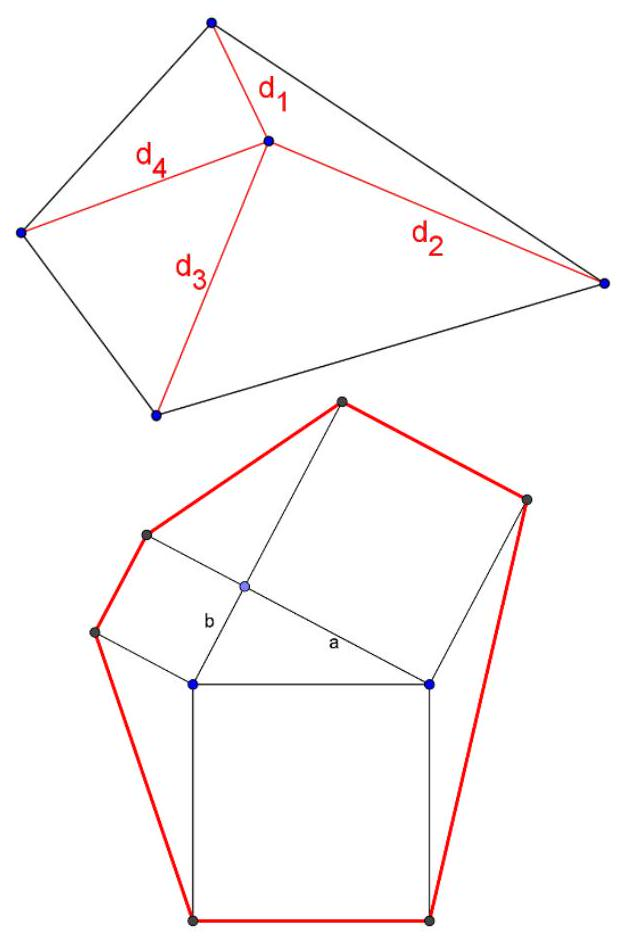
\includegraphics[max width=\textwidth, center]{2024_11_21_59b0c2c0bc9b0a979429g-1(1)}


\end{document}